
%%% Local Variables:
%%% mode: latex
%%% TeX-master: t
%%% End:
\section{空间数据绘图系统}

\begin{frame}[c]{\subsecname}{}
      \begin{ornamentblock}%\hspace*{\parindent}
\hspace*{2em}我们借助于外感官(我们意识的一种性质)表象给我们自己外面的对象,这些对
象毫无例外的在空间里面。这些对象的形状、大小、以及它们相互间的关系是在
空间里被规定的或能够在空间里被规定的。\\
\hspace*{2em}空间不是一个从外部经验得来的经验概念。因为为使着某种感觉与我以外的某些
东西发生关系,以及同样地为着我能把那些感觉表象为互相在外、互相靠近,从
而不只是彼此不同,并且是在不同的地方,这样就一定要以空间观念为前提。\\
          \rightline{\textemdash《康德·纯粹理性批判》}
      \end{ornamentblock}
\end{frame}

\subsection{GIS和R}
\begin{frame}[t]{\subsecname}{}
\begin{itemize}
\item GIS的非正式定义\footnotemark[1]:一组强大的工具集,可以用来收集、存储、任意检索、转换和
显示\emphText{来自真实世界有特殊用途的空间数据}
\item R虽然能够分析并提供数据可视化,但是并没有能力从其他数据中区分出空间数据;因此一组R开发者共同
实现了R的\emphText{空间数据类包sp}\footnotemark[2],它新增了用于空间数据类和方法的R功能
\end{itemize}

\only<2>{
\begin{block}{\small 空间数据类的优势}
  \begin{itemize} \footnotesize
  \item[\PencilLeftDown] 从空间分析包中转换数据更加容易
  \item[\PencilLeftDown] 提供GIS接口包,可以读写外部GIS格式数据
  \item[\PencilLeftDown] 实现空间数据组织、绘图、打印的方法
  \item[\PencilLeftDown] 能够对绘图进行地图修饰(参考网格、指北针、比例尺)
  \end{itemize}
\end{block}}

\footnotetext[1]{
Burrough, P. A. and McDonnell, R. A. (1998). \emph{Principles of Geographical
Information Systems}. Oxford University Press, Oxford.}
\footnotetext[2]{
Pebesma, E. J. and Bivand, R. S. (2005). \emph{Classes and methods for spatial
data in R}. R News, 5(2):9–13.}
\end{frame}

\subsection{R的空间数据类}
\begin{frame}[t]{\subsecname}{}
\begin{itemize}
\item<1-> sp包从2005年开始提交CRAN,主要创始人是挪威经济学院教授
\href{https://www.nhh.no/en/employees/faculty/roger-bivand/}{\uline{Roger Bivand}}和
慕尼黑大学教授\href{https://www.uni-muenster.de/Geoinformatics/en/institute/staff/index.php/119/Edzer_Pebesma}{\uline{Edzer Pebesma}};目前项目负责人是Edzer,并有稳定的开发团队和成熟的讨论组
\item<2-> sp包未包含在base包中,需要单独下载使用
\item<3-> 目前绝大多数空间数据相关的包都会以sp包为基础来编写
\end{itemize}

\begin{overlayarea}{\textwidth}{\textheight}
\only<1>{
\begin{figure}
\begin{columns}
    \begin{column}{.5\textwidth}\centering
        
\includegraphics[width=0.7\columnwidth]{roger_bivand.jpg}
    \end{column}

    \begin{column}{.5\textwidth}\centering
        
\includegraphics[width=0.55\columnwidth]{edzer_pebesma.jpg}
    \end{column}
  \end{columns}
\caption{sp包的两位主要作者.左边是Roger Bivand,右边是Edzer Pebesma}
\end{figure}}

\only<3>{
\begin{figure}
    \centering
    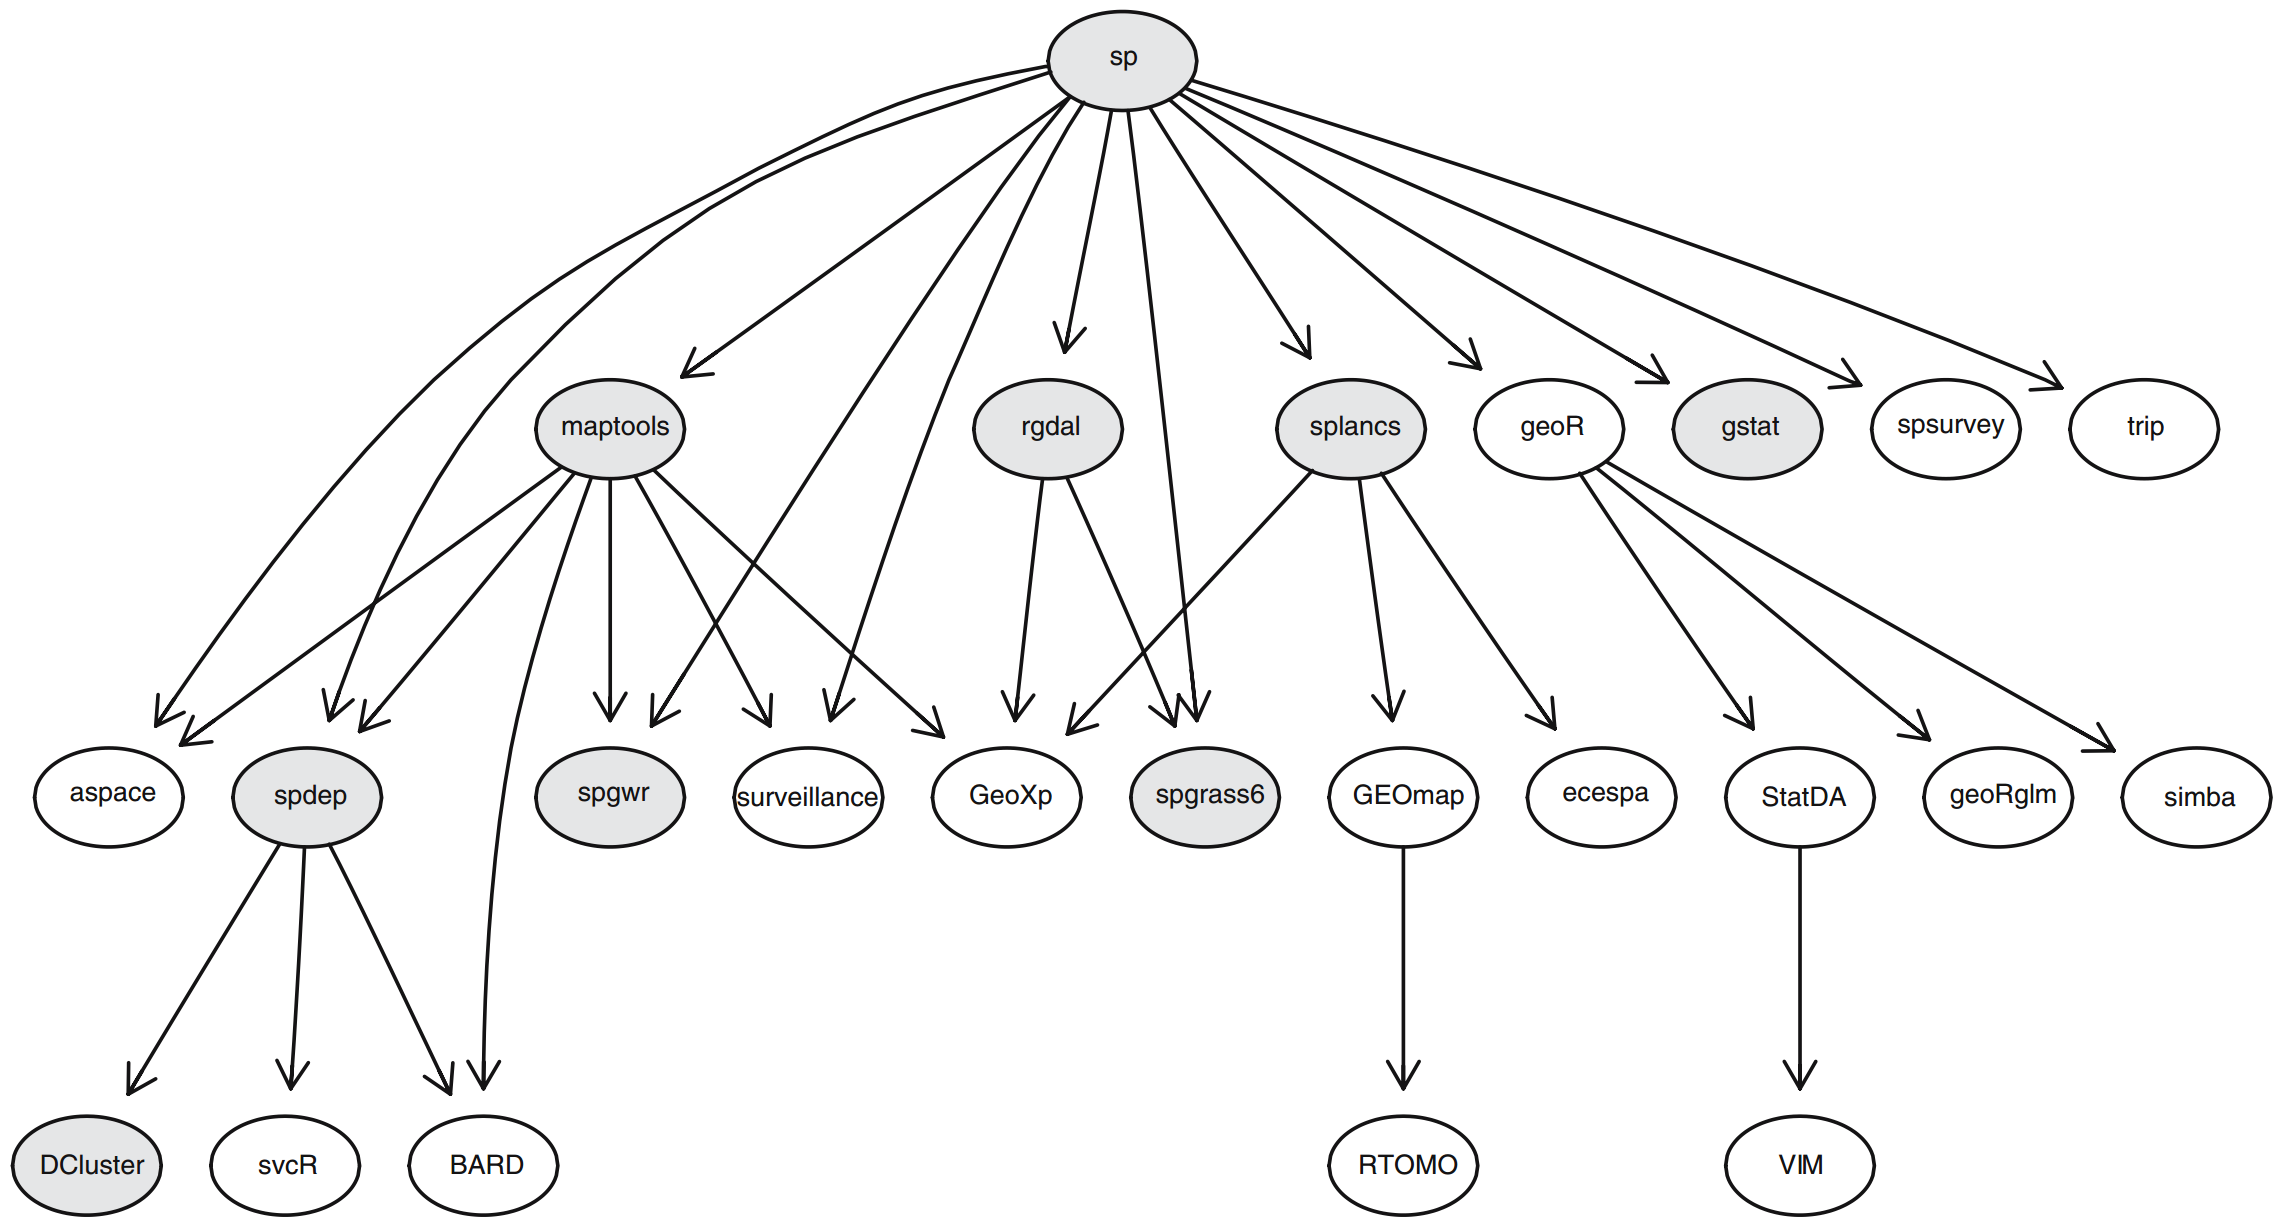
\includegraphics[width=0.8\columnwidth]{sp_depend.png}
    \caption{直接或间接基于sp包开发的程序包}
\end{figure}}
\end{overlayarea}
\end{frame}

\begin{frame}[t,fragile]{\subsecname}{}
\begin{itemize}
\item<1-> sp包提供的空间类是\emphText{基于S4方法编写的},其\emphText{基类是Spatial}
\item<2-> Spatial类包括两个属性(slot),一个是matrix类型的\emphText{约束盒}(bbox),
另一个是CRS类型的\emphText{坐标参考系统}(proj4string)
\item<3-> 约束盒是列名为\emphText{c('min','max')}的坐标矩阵,至少有两列,一列指向东(x轴),一列
指向北(y轴);CRS类只有一个属性,其值是一个\emphText{\href{http://proj4.org/}{\uline{PROJ.4}}开源CRS格式的字符串}
\end{itemize}

\begin{overlayarea}{\textwidth}{\textheight}
\begin{onlyenv}<2>
\begin{rcode}
> library(sp)
> getClass("Spatial")
Class "Spatial" [package "sp"]

Slots:
                              
Name:         |\colorbox{green}{bbox}| |\colorbox{green}{proj4string}|
Class:      matrix         CRS

Known Subclasses: 
Class "SpatialPoints", directly
Class "SpatialMultiPoints", directly
Class "SpatialGrid", directly
Class "SpatialLines", directly
Class "SpatialPolygons", directly
Class "SpatialPointsDataFrame", by class "SpatialPoints", distance 2
Class "SpatialPixels", by class "SpatialPoints", distance 2
Class "SpatialMultiPointsDataFrame", by class "SpatialMultiPoints", distance 2
Class "SpatialGridDataFrame", by class "SpatialGrid", distance 2
Class "SpatialLinesDataFrame", by class "SpatialLines", distance 2
Class "SpatialPixelsDataFrame", by class "SpatialPoints", distance 3
Class "SpatialPolygonsDataFrame", by class "SpatialPolygons", distance 2
\end{rcode}
\end{onlyenv}

\begin{onlyenv}<3>
\begin{rcode}
# 定义约束盒
> bb <- matrix(c(114.25, 22.45, 114.85, 23.16), ncol = 2, dimnames = list(NULL, c("min", "max")))
# 新建一个Spatial对象,CRS对象是经纬度坐标系统
> Spatial(bb, proj4string = CRS("+proj=longlat"))
An object of class "Spatial"
Slot "bbox":
        min    max
[1,] 114.25 114.85
[2,]  22.45  23.16

Slot "proj4string":
CRS arguments: +proj=longlat
\end{rcode}
\end{onlyenv}
\end{overlayarea}
\end{frame}

\begin{frame}[t,fragile]{\subsecname}{SpatialPoints类}
\begin{itemize}
\item<1-> \emphText{SpatialPoints}是sp包中用来表达空间点的类
\item<2-> 相比Spatial类,SpatialPoints类扩展了一个matrix类型的属性\emphText{coords}来存储点坐标矩阵
\end{itemize}

\begin{overlayarea}{\textwidth}{\textheight}
\begin{onlyenv}<2->
\begin{rcode}
> getClass("SpatialPoints")
Class "SpatialPoints" [package "sp"]

Slots:
                                          
Name:       |\colorbox{green}{coords}|        bbox proj4string
Class:      matrix      matrix         CRS

Extends: "Spatial"

Known Subclasses: 
Class "SpatialPointsDataFrame", directly
Class "SpatialPixels", directly
Class "SpatialPixelsDataFrame", by class "SpatialPixels", distance 2
\end{rcode}
\end{onlyenv}

\begin{onlyenv}<3>
\begin{rcode}
# 读取格式化文件到一个data.frame类型对象CRAN\_df,包含位置经纬度坐标
> CRAN_df <- read.table("data/CRAN051001a.txt", header = TRUE)
# 将经纬度坐标构建一个新的matrix类型对象CRAN\_mat
> CRAN_mat <- cbind(CRAN_df$long, CRAN_df$lat)

# 构建一个CRS对象llCRS 
llCRS <- CRS("+proj=longlat +ellps=WGS84")
# 构建SpatialPoints对象
CRAN_sp <- |\colorbox{green}{SpatialPoints}|(CRAN_mat, proj4string = llCRS)
\end{rcode}
\end{onlyenv}
\end{overlayarea}
\end{frame}

\begin{frame}[t,fragile]{\subsecname}{SpatialPoints类}
\begin{itemize}
\item<1-> \emphText{SpatialPointsDataFrame}类将SpatialPoints对象转换为类似data.frame数据结构
\item<2-> SpatialPointsDataFrame类通过coords行名和data.frame行名的对应顺序来构建,
\emphText{可以用于在空间信息后面挂载属性信息}
\item<4-> SpatialPointsDataFrame对象有两个索引,一个用于空间对象,另一个用于列
\end{itemize}

\begin{overlayarea}{\textwidth}{\textheight}
\begin{onlyenv}<1>
\begin{rcode}
> getClass("SpatialPointsDataFrame")
Class "SpatialPointsDataFrame" [package "sp"]

Slots:                                                                  

Name:         data  coords.nrs      coords        bbox proj4string
Class:  data.frame     numeric      matrix      matrix         CRS

Extends: 
Class "SpatialPoints", directly
Class "Spatial", by class "SpatialPoints", distance 2
\end{rcode}
\begin{figure}[ht]\vspace{-10pt}
  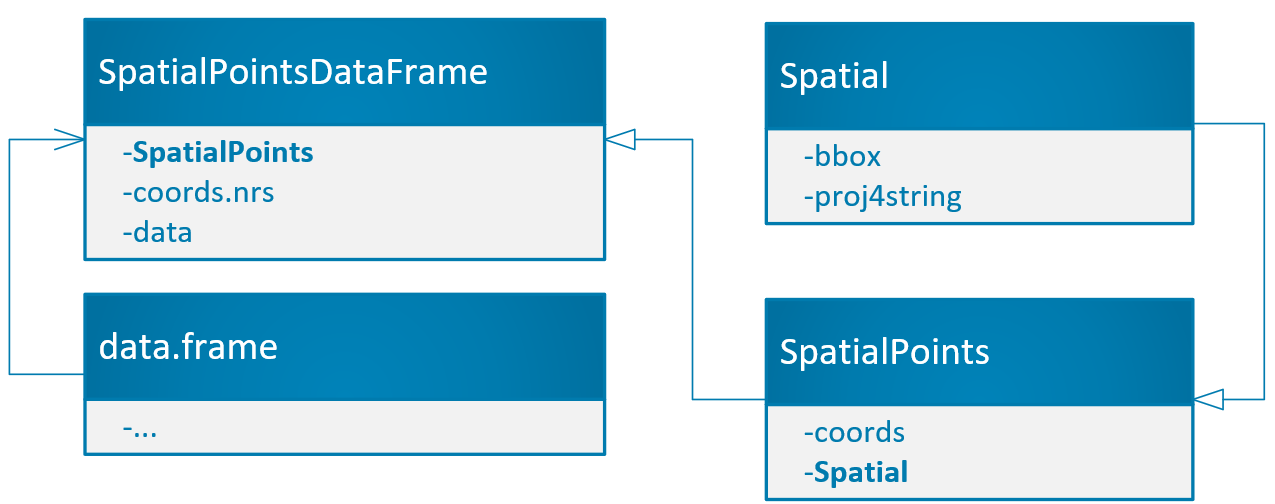
\includegraphics[width=0.6\columnwidth]{spatialpointsdataframe_class.png}
\end{figure}
\end{onlyenv}

\begin{onlyenv}<2>
\begin{rcode}
# 将matrix的序号作为行名
> row.names(CRAN_mat) <- 1:nrow(CRAN_mat)
> str(CRAN_mat)
 num [1:54, 1:2] 153 145 16.3 -49.3 -42.9 ...
 - attr(*, "dimnames")=List of 2
  ..$ : chr [1:54] "1" "2" "3" "4" ...
  ..$ : NULL

# 构建Spatialpoints对象CRAN\_spdf1,match.ID=TURE表示根据CRAN\_mat行名和CRAN\_df行名要对应
> CRAN_spdf1 <- |\colorbox{green}{SpatialPointsDataFrame}|(coords=CRAN_mat, data=CRAN_df, proj4string=llCRS, match.ID=TRUE)
\end{rcode}
\end{onlyenv}

\begin{onlyenv}<3>
\begin{rcode}
# 构建的新对象在空间信息基础上挂载了属性信息long、lat、place、north、east和loc
> str(CRAN_spdf1)
Formal class 'SpatialPointsDataFrame' [package "sp"] with 5 slots
  ..@ data       :'data.frame': 54 obs. of  6 variables:
  .. ..$ place: Factor w/ 52 levels "Aalborg","Aizu",..: 9 30 50 15 49 39 36 40 12 46 ...
  .. ..$ north: Factor w/ 52 levels "20d45'S","22d43'S",..: 8 18 41 7 1 3 2 4 43 29 ...
  .. ..$ east : Factor w/ 51 levels "0d10'W","118d15'W",..: 19 16 20 35 31 32 34 33 11 39 ...
  .. ..$ loc  : Factor w/ 30 levels "Australia","Austria",..: 1 1 2 3 3 3 3 3 4 19 ...
  .. ..$ long : num [1:54] 153 145 16.3 -49.3 -42.9 ...
  .. ..$ lat  : num [1:54] -27.5 -37.8 48.2 -25.4 -20.8 ...
  ..@ coords.nrs : num(0) 
  ..@ coords     : num [1:54, 1:2] 153 145 16.3 -49.3 -42.9 ...
  .. ..- attr(*, "dimnames")=List of 2
  .. .. ..$ : chr [1:54] "1" "2" "3" "4" ...
  .. .. ..$ : chr [1:2] "coords.x1" "coords.x2"
  ..@ bbox       : num [1:2, 1:2] -123 -37.8 153 57
  .. ..- attr(*, "dimnames")=List of 2
  .. .. ..$ : chr [1:2] "coords.x1" "coords.x2"
  .. .. ..$ : chr [1:2] "min" "max"
  ..@ proj4string:Formal class 'CRS' [package "sp"] with 1 slot
  .. .. ..@ projargs: chr "+proj=longlat +ellps=WGS84"  
\end{rcode}
\end{onlyenv}

\begin{onlyenv}<4>
\begin{rcode}
# 根据序号进行空间对象索引
> CRAN_spdf1[10, ]
          coordinates   place   north    east           loc      long   lat
10 (-79.38333, 43.65) Toronto 43d39'N 79d23'W Ontario (CAN) -79.38333 43.65

# 根据列进行索引,用法和data.frame类型的列索引一样,有两种等价的方法
> str(CRAN_spdf1$loc)
 Factor w/ 30 levels "Australia","Austria",..: 1 1 2 3 3 3 3 3 4 19 ...
> str(CRAN_spdf1[["loc"]])
Factor w/ 30 levels "Australia","Austria",..: 1 1 2 3 3 ...
\end{rcode}
\end{onlyenv}
\end{overlayarea}
\end{frame}

\begin{frame}[t,fragile]{\subsecname}{SpatialLines类}
\begin{itemize}
\item<1-> 普通线对象在sp包中用\emphText{Line}类来表达,并且一系列Line构成\emphText{Lines}类
\item<2-> 但是Line和Lines不包含约束盒和坐标系统,所以sp包提供\emphText{SpatialLines}类用来专门表达空间线对象
\item<2-> SpatialLines类继承自Spatial类,除bbox和CRS之外,
还扩展了一个list类型的属性\emphText{lines}用来存储Lines对象
\end{itemize}

\begin{overlayarea}{\textwidth}{\textheight}
\begin{onlyenv}<1>
\begin{rcode}
# Line类包含属性coords用来存储构成线的连续点坐标矩阵
> getClass("Line")
Class "Line" [package "sp"]

Slots:
             
Name:  |\colorbox{green}{coords}|
Class: matrix

Known Subclasses: "Polygon"

# Lines类包含一个属性Lines用来存储一系列Line对象,另一个slot ID用来标识Lines对象的唯一性
> getClass("Lines")
Class "Lines" [package "sp"]

Slots:
                          
Name:      |\colorbox{green}{Lines}|        |\colorbox{green}{ID}|
Class:      list character
\end{rcode}
\end{onlyenv}

\begin{onlyenv}<2>
\begin{rcode}
> getClass("SpatialLines")
Class "SpatialLines" [package "sp"]

Slots:
                                          
Name:        |\colorbox{green}{lines}|        bbox proj4string
Class:        list      matrix         CRS

Extends: "Spatial"

Known Subclasses: "SpatialLinesDataFrame"
\end{rcode}
\end{onlyenv}
\end{overlayarea}
\end{frame}

\begin{frame}[t,fragile]{\subsecname}{SpatialLines类}
\begin{itemize}
\item<1-> sp包也提供了\emphText{SpatialLinesDataFrame}类将SpatialLines对象转换为类似data.frame数据结构
\end{itemize}

\begin{rcode}
> getClass("SpatialLinesDataFrame")
Class "SpatialLinesDataFrame" [package "sp"]

Slots:
                                                      
Name:         data       lines        bbox proj4string
Class:  data.frame        list      matrix         CRS

Extends: 
Class "SpatialLines", directly
Class "Spatial", by class "SpatialLines", distance 2
\end{rcode}
\begin{figure}[ht]
  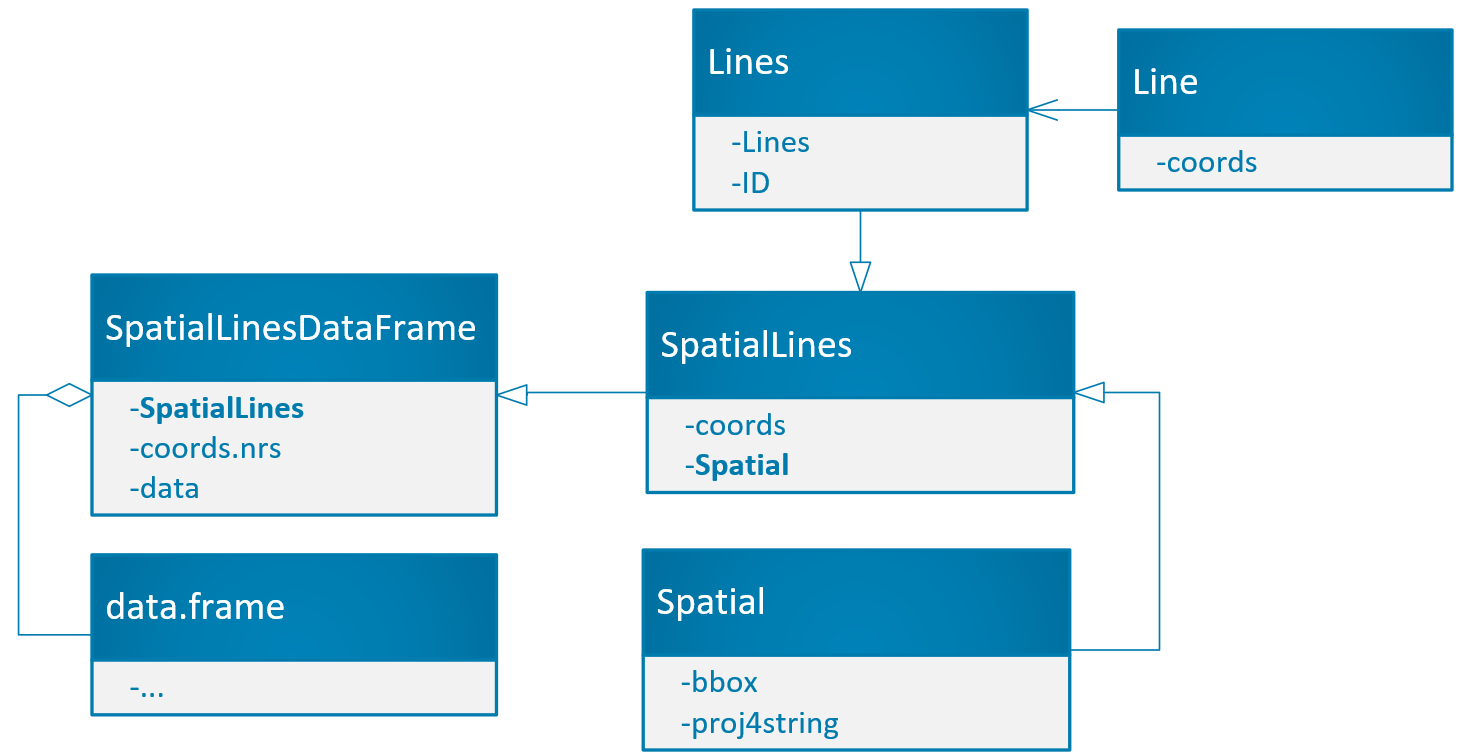
\includegraphics[width=0.7\columnwidth]{spatiallinesdataframe_class.png}
\end{figure}
\end{frame}
\subsection{空间数据的导入导出}

\subsection{空间数据可视化}